\documentclass[tikz,border=6pt]{standalone}
\usepackage{pgfplots}
\pgfplotsset{compat=1.18}
\begin{document}
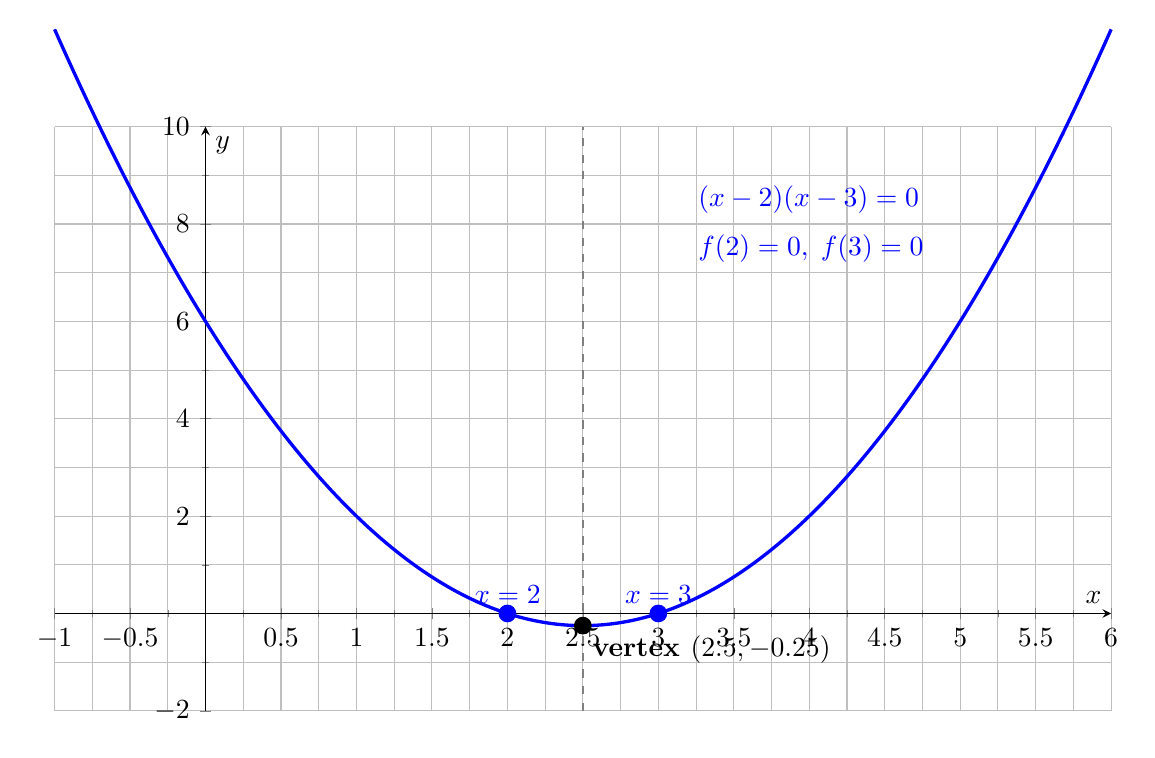
\begin{tikzpicture}
\begin{axis}[
  width=15cm,height=9cm,
  xmin=-1,xmax=6,ymin=-2,ymax=10,
  axis lines=middle,
  xlabel={$x$},ylabel={$y$},
  grid=both,minor tick num=1,
  samples=240,clip=false
]
\addplot[blue,very thick,domain=-1:6]{x^2-5*x+6};
\addplot[gray,dashed,thick] coordinates {(2.5,-2) (2.5,10)};
\addplot[blue,only marks,mark=*,mark size=3pt] coordinates {(2,0) (3,0)};
\addplot[black,only marks,mark=*,mark size=3pt] coordinates {(2.5,-0.25)};
\node[blue,font=\bfseries,anchor=south] at (axis cs:2,0) {$x=2$};
\node[blue,font=\bfseries,anchor=south] at (axis cs:3,0) {$x=3$};
\node[black,font=\bfseries,anchor=north west] at (axis cs:2.5,-0.25) {vertex $(2.5,-0.25)$};
\node[blue,font=\bfseries,anchor=west] at (axis cs:3.2,8.5) {$(x-2)(x-3)=0$};
\node[blue,font=\bfseries,anchor=west] at (axis cs:3.2,7.5) {$f(2)=0,\;f(3)=0$};
\end{axis}
\end{tikzpicture}
\end{document}
